\chapter{Wstęp teoretyczny}
\label{ch:wstept}

$TODO$
Cooperative Pathfinding
David Silver
Cooperative Pathfinding is a multi-agent path planning problem where agents must find non-colliding routes to separate destinations, given full information about the routes of other agents. This paper presents three new algorithms for efficiently solving this problem, suitable for use in Real-Time Strategy games and other real-time environments. The algorithms are decoupled approaches that break down the problem into a series of single-agent searches. Cooperative A* (CA*) searches space-time for a non-colliding route. Hierarchical Cooperative A* (HCA*) uses an abstract heuristic to boost performance. Finally, Windowed Hierarchical Cooperative A* (WHCA*) limits the space-time search depth to a dynamic window, spreading computation over the duration of the route. The algorithms are applied to a series of challenging, maze-like environments, and compared to A* with Local Repair (the current video-games industry standard). The results show that the new algorithms, especially WHCA*, are robust and efficient solutions to the Cooperative Pathfinding problem, finding more successful routes and following better paths than Local Repair A*.

Kooperacyjne znajdowanie tras (ang. Cooperative Pathfinding) jest problemem planowania w układzie wieloagentowym, gdzie agenci muszą znaleźć bezkolizyjne drogi do swoich, osobnych celów. Planowanie to odbywa się mając pełną informację o środowisku oraz trasach pozostałych agentów. 


Przedmiotem niniejszej pracy jest przegląd metod rozwiązujacych zagadnienie planowania bezkolizyjnych tras dla wielu robotów. Stanowi to wstęp do zaprojektowania algorytmu i implementacji oprogramowania pozwalającego na symulację jego działania w praktyce (tzn. na przykładzie $TODO$).

$TODO$ nie ma algorytmów do planowania tras w środowiskach ciasnych korytarzy (duża liczba przeszkód, częsty problem blokowania w wąskich korytarzach, zakleszczenie)
$TODO$ Problem do rozwiązania: Dane: mapa otoczenia i przestrzeń konfiguracyjna, określone położenie początkowe i cel dla zespołu robotów; Zadanie: Wyznaczenie możliwie najkrótszej bezkolizyjnej trasy dla wszystkich robotów.
$TODO$ nie otwarte środowisko, ale zamknięte, z dużą liczbą przeszkód

\begin{itemize}
	\item Koordynacja ruchu robotów jest jednym z fundamentalnych problemów dla systemów wielu robotów.
	\item Popularne podejścia omijające planowanie w wysoko wymiarowej zbiorowej przestrzeni konfiguracyjnej to techniki rozproszone i priorytetowane.
	\item Pomimo, że te metody są bardzo efektywne, mają dwie główne wady:
	\begin{enumerate}
		\item nie są zupełne - czasami nie udaje się znaleźć rozwiązania, nawet gdy istnieje.
		\item Wynikowe rozwiązania są często nieoptymalne.
	\end{enumerate}
	\item Ponadto nie mówią, jak przypisywać priorytety do pojedynczych robotów.
	\item W tym artykule przedstawiono metodę do optymalizowania układu priorytetów dla rozproszonych i priorytetowanych technik planowania.
	\item Proponowana metoda wykonuje randomizowane przeszukiwanie z techniką hill-climbing do znalezienia rozwiązania i do skrócenia całkowitej długości ścieżek.
	\item Technika została zaimplemenotwana i przetestowana na prawdziwych robotach oraz w rozległych testach symulacyjnych.
	\item Wyniki eksperyentu pokazały, że metoda potrafi znacząco zmniejszyć liczbę niepowodzeń i znacznie zmniejszyć całkowitą długość tras dla różnych priorytetowanych i rozproszoncyh metod planowania dróg, nawet dla dużych zespołów robotów.
\end{itemize}

\section{Przestrzeń konfiguracyjna}
Przestrzeń konfiguracyjna to formalna, matematyczna przestrzeń będąca zbiorem możliwych stanów danego układu fizycznego.
W zależności od rodzaju i liczby wyróżnionych parametrów stanu przestrzenie konfiguracyjne mogą mieć wiele wymiarów.

\section{Metoda hill-climbing}
Metoda hill-climbing jest rodzajem matematycznej optymalizacji, lokalną metodą przeszukiwania.
Jest to iteracyjny algorytm, który zaczyna w wybranym rozwiązaniu problemu, następnie próbuje znaleźć lepsze rozwiązanie poprzez przyrostowe zmiany pojedynczych elementów rozwiązania.
Jeśli zmiana przynosi lepsze rozwiązanie, jest wprowadzana do nowego rozwiązania.
Kroki algorytmu powtarzane są dopóki żadne ``udoskonalenia'' nie mogą już być znalezione.

\section{Metody planowania tras}
Spośród metod wykorzystywanych do planowania tras dla wielu robotów można wyróżnić dwie grupy:
\begin{itemize}
	\item zcentralizowane - drogi wyznaczane są dla wszystkich agentów na raz (jednocześnie). Metody te potrafią znaleźć optymalne rozwiązanie, ale często mają bardzo dużą złożoność obliczeniową, dlatego wykorzystywane są heurystyki
	\item rozproszone (ang. decoupled) - dla każdego robota droga wyznaczana jest osobno, w określonej kolejności, następnie rozwiązywane są konflikty (kolizje dróg), może nie znaleźć istniejącego rozwiązania. Metoda najczęściej wiąże się z koniecznością przydzielenia robotowi priorytetu, co stanowi istotny problem, gdyż od wyboru priorytetów może zależeć zupełność algorytmu.
\end{itemize}

\subsection{Metody zcentralizowane}
Zalety:
\begin{itemize}
	\item Planowanie w zbiorowej przestrzeni konfiguracyjnej
	\item Wyznaczenie {\bf optymalnego} rozwiązania
	\item W praktyce: Heurystyka radzi sobie z ogromną złożonością przestrzeni konfiguracyjnej
\end{itemize}
Podejścia (bez gwarancji optymalności):
\begin{itemize}
	\item Potential field techniques - Metoda potencjałowa
	\item Roadmap methods % przeszukiwanie grafu połączeń - Dijkstry
\end{itemize}

% decoupled - rozproszony, odzielny
\subsection{Podejście "Decoupled"}
Algorytm (niezupełny):
\begin{enumerate}
	\item Wyznaczenie optymalnej ścieżki dla każdego robota {\bf niezależnie}
	\item Przydział priorytetów (opcjonalne)
	\item Próba rozwiązania możliwych konfliktów między ścieżkami
\end{enumerate}
% może nie znaleźć istniejącego rozwiązania
Podejścia:
\begin{itemize}
	\item Path coordination
	\item Planning in the configuration time-space: % TODO tłumaczenie
		\begin{itemize}
			\item V-Graph algorithm
			\item Potential fields
			\item A*
		\end{itemize}
\end{itemize}

\subsubsection{Path coordination}
Idea:
\begin{itemize}
	\item Utrzymanie robotów na ich indywidualnych, optymalnych ścieżkach
	\item Pozwolenie na zatrzymanie się, ruch naprzód, a nawet cofanie się, ale tylko {\bf wzdłuż trajektorii} w celu uniknięcia kolizji
\end{itemize}
W praktyce:
\begin{itemize}
	\item Wymagany wariant z ustaleniem priorytetów
	\item Złożoność $O(n \cdot m \cdot log(m))$, m - maksymalna liczba stanów podczas planowania % n - liczba robotów, m - maksymalna liczba stanów podczas planowania w konfiguracji time-space
\end{itemize}

\subsubsection{Konieczność wyboru priorytetów}
\begin{figure}[htp]
	\centering
	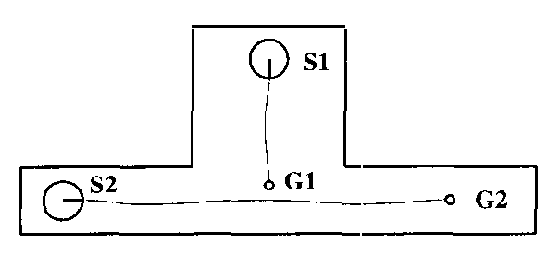
\includegraphics[width=\textwidth,height=0.4\textheight,keepaspectratio]{img/article1/fig1}
	\caption{Sytuacja, w której żadne rozwiązanie nie zostanie znalezione, jeśli robot 1 ma wyższy priorytet niż robot 2}
\end{figure}

\subsubsection{Zastosowanie A* w planowaniu dróg dla wielu robotów}
Algorytm:
\begin{itemize}
	\item Przypisanie priorytetów do poszczególnych robotów
	\item Wykonywanie kroków A* z rozpatrywaniem czasu i przestrzeni - podział otoczenia na siatkę pól, zapisywanie prawdopodobieństwa zajętości pola w danej chwili
\end{itemize}
Złożoność:
\begin{itemize}
	\item $O(n \cdot m \cdot log(m))$, m - maksymalna liczba stanów podczas planowania (lista otwartych) % n - liczba robotów, m - maksymalna liczba stanów podczas planowania w konfiguracji time-space = maksymalny rozmiar listy OPEN
\end{itemize}
% jak działa A*, A* sprowadza się do Dijkstry

\subsubsection{Wpływ układu priorytetów na długość tras}
\begin{figure}[htp]
	\centering
	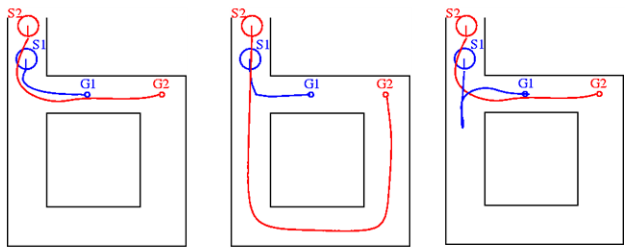
\includegraphics[width=\textwidth,height=0.6\textheight,keepaspectratio]{img/article1/ppt6}
	\caption{Niezależne planowanie optymalnych tras dla 2 robotów; suboptymalne rozwiązanie, gdy robot 1 ma wyższy priorytet; rozwiązanie, gdy robot 2 ma wyższy priorytet}
\end{figure}

\section{Wybór priorytetów}
\subsubsection{Elastyczny dobór priorytetów}
Obecne techniki pozostawiają dowolny wybór priorytetów lub korzystają z ustalonego z góry stałego układu kolejności robotów. \\
\vspace{1em}
{\bf Cel:} \\
Połączyć ze sobą planowanie tras i przypisanie priorytetów, wykorzystując randomizowane techniki.

\subsubsection{Poszukiwanie układu priorytetów mających rozwiązanie}
% pierwsza wersja algorytmu - nieoptymalna
\begin{figure}[htp]
	\centering
	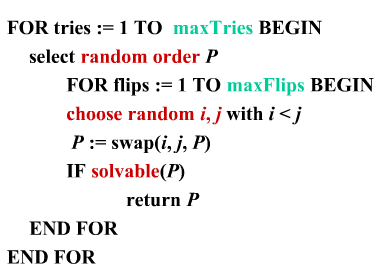
\includegraphics[width=\textwidth,height=0.6\textheight,keepaspectratio]{img/article1/algorytm}
\end{figure}
Prosta technika losująca układ priorytetów (kolejności robotów) daje dobre rezultaty, ale często duża liczba iteracji jest konieczna do uzyskania rozwiązania.

\section{Rezultaty}
\subsection{Ocena metody przez Eksperyment}
Testy symulacyjne:
\begin{itemize}
	\item Zastosowanie naszego algorytmu wyboru priorytetów:
		\begin{itemize}
			\item A* in the configuration time-space
			\item path coordination method
		\end{itemize}
	\item Użycie 2 różnych środowisk (acykliczne / cykliczne)
	\item Losowe generowanie punktów startu i celu
\end{itemize}

\subsubsection{Zoptymalizowany algorytm wyznaczania priorytetów}
\begin{figure}[htp]
	\centering
	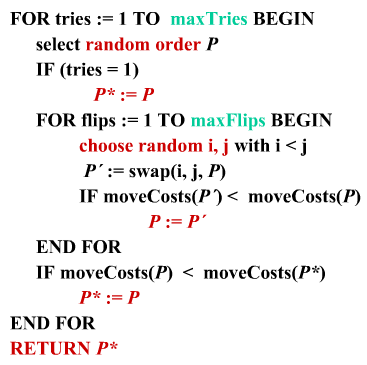
\includegraphics[width=\textwidth,height=0.7\textheight,keepaspectratio]{img/article1/ppt-alg2}
\end{figure}
% ZALETA: można przerwać w dowolnym momencie

\section{Podusmowanie}
\subsection{Wnioski}
\begin{itemize}
	\item Zaprezentowano metodę doboru priorytetów dla rozproszonych metod planowania dróg dla grupy robotów mobilnych.
	\item Zaproponowane podejście to randomizowana metoda, która cyklicznie zamienia kolejność robotów w celu znalezienia sekwencji, dla której można wyznaczyć plan dróg oraz w celu minimalizacji całkowitej długości tras.
	\item Jest to algorytm, który może być zatrzymany w dowolnym momencie i może zawsze zwrócić obecnie najlepsze rozwiązanie.
	\item Metoda została zaimplementowana i przetestowana na rzeczywistych robotach i w rozległych testach symulacyjnych dla dwóch różnych metod planowania dróg oraz dla dużej liczby robotów.
	\item Wyniki eksperyentu pokazały, że metoda potrafi znacząco zmniejszyć liczbę niepowodzeń (gdy żadne rozwiązanie nie zostaje znalezione) i znacznie zmniejszyć całkowitą długość tras.
\end{itemize}
